\documentclass{article}

\title{CPSC 2150 HW5 Writeup}
\author{Rex Oliver}
\date{April 24 2019}

\usepackage{pdfpages} 
\begin{document}

\begin{titlepage}
  \maketitle
\end{titlepage}

% \newcommand{\testgrid}[6][][][][][][]

\section{Requirements Analysis}
Functional Requirements:
\begin{itemize}
  \item As a user, I can choose how many rows should be on the board.
  \item As a user, I can choose how many columns should be on the board.
  \item As a user, I can choose how many in a row to win.
  \item As a user, I can choose what column to place my marker in.
  \item As a user, I can choose to play again or not.
  \item As a user, I can view the prompt that asks the user to make a move.
  \item As a user, I can view the prompt that asks the user to play again or
    not.
  \item As a user, I can view the prompt that asks the user how many rows should be on the board.
  \item As a user, I can view the prompt that asks the user how many column should be on the board.
  \item As a user, I can view the prompt that asks the user how many in a row to win? 
  \item As a user, I can view the printed board with updated moves each turn.
  \item As a user, I can be notified of a win.
  \item As a user, I will not lose a turn for bad input.
  \item As a user, I can view the prompt that asks the user how many players to play the game.
  \item As a user, I can choose how many players to play in the game.
\end{itemize}
Non-functional Requirements
\begin{itemize}
\item The system must run on the School of Computing Linux Systems.
\item The system must be written in Java.
\item The system uses a GUI.  
\end{itemize}  

\section{Design}
\paragraph{}
UML Diagram on next page, with the test cases listed right after.    

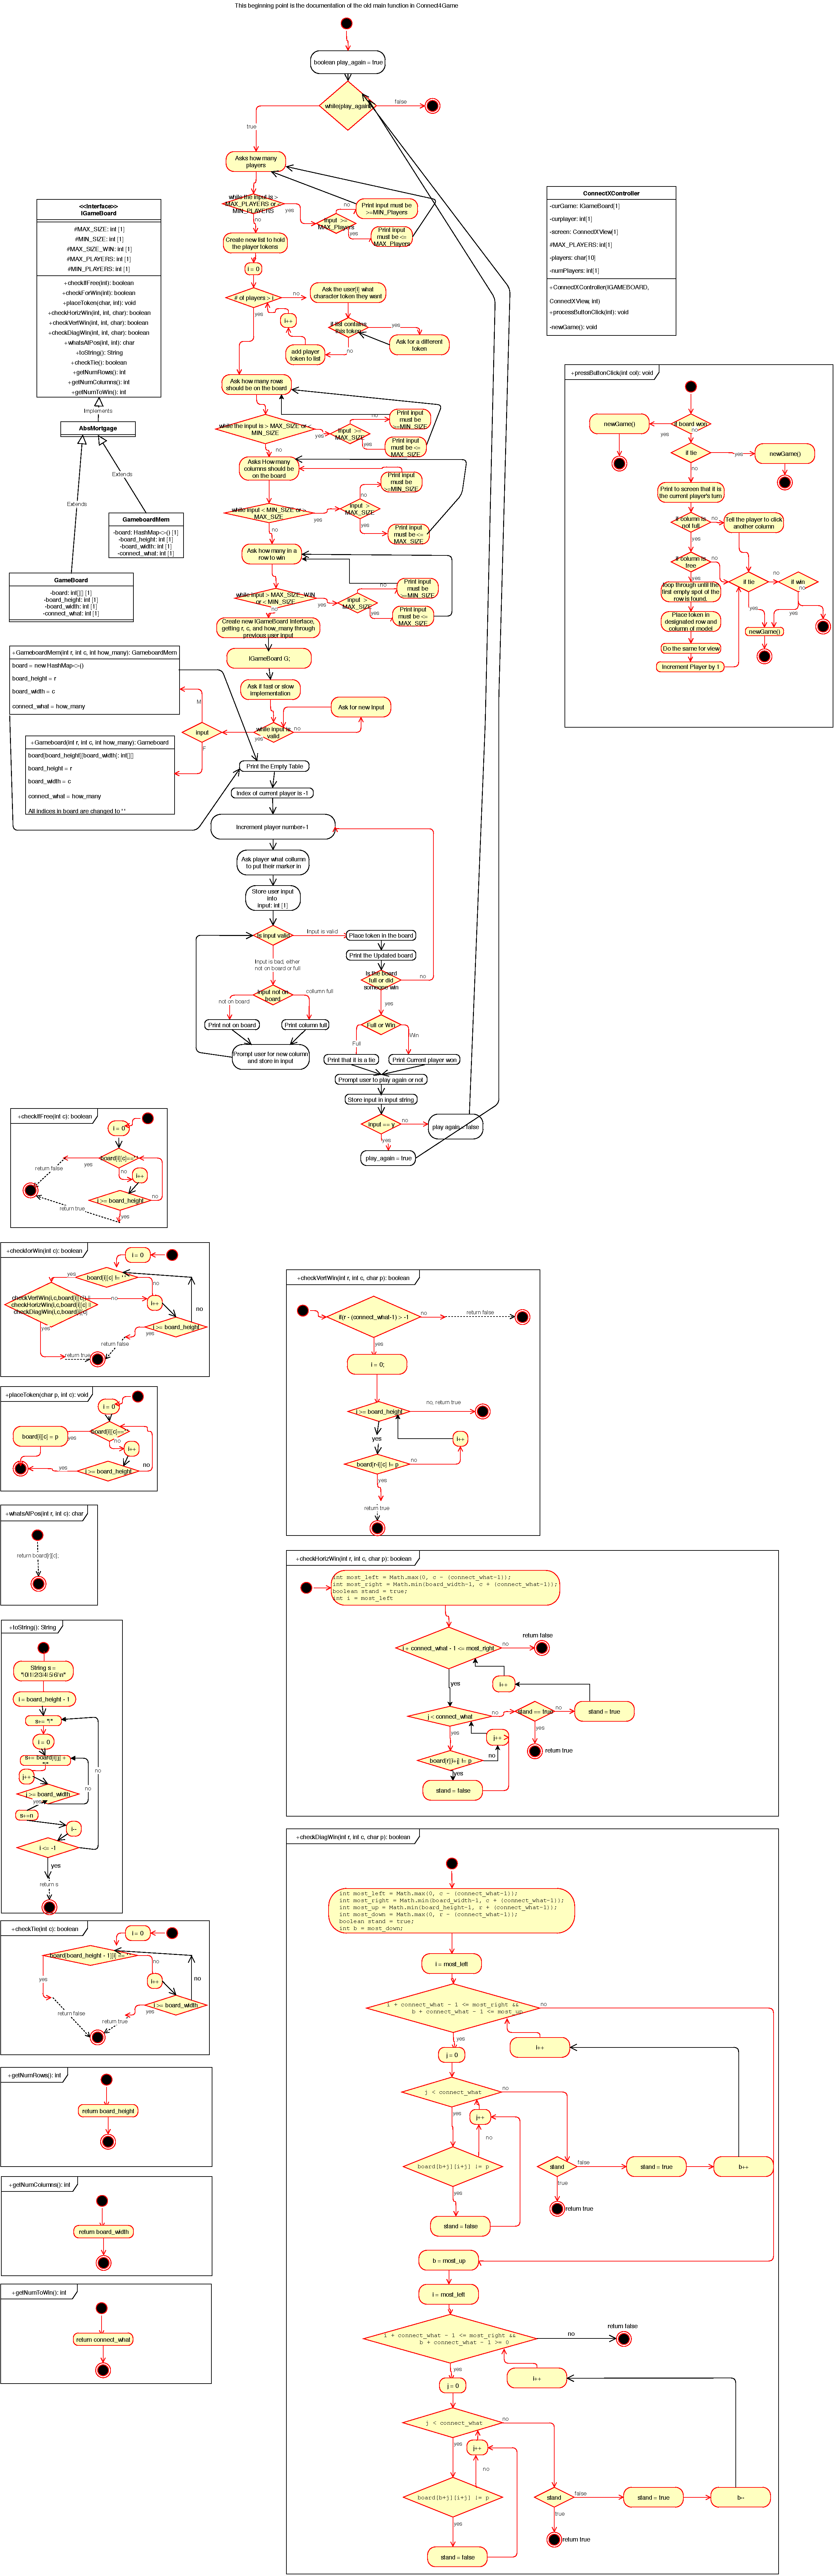
\includepdf[pages={1}]{2150HW5}
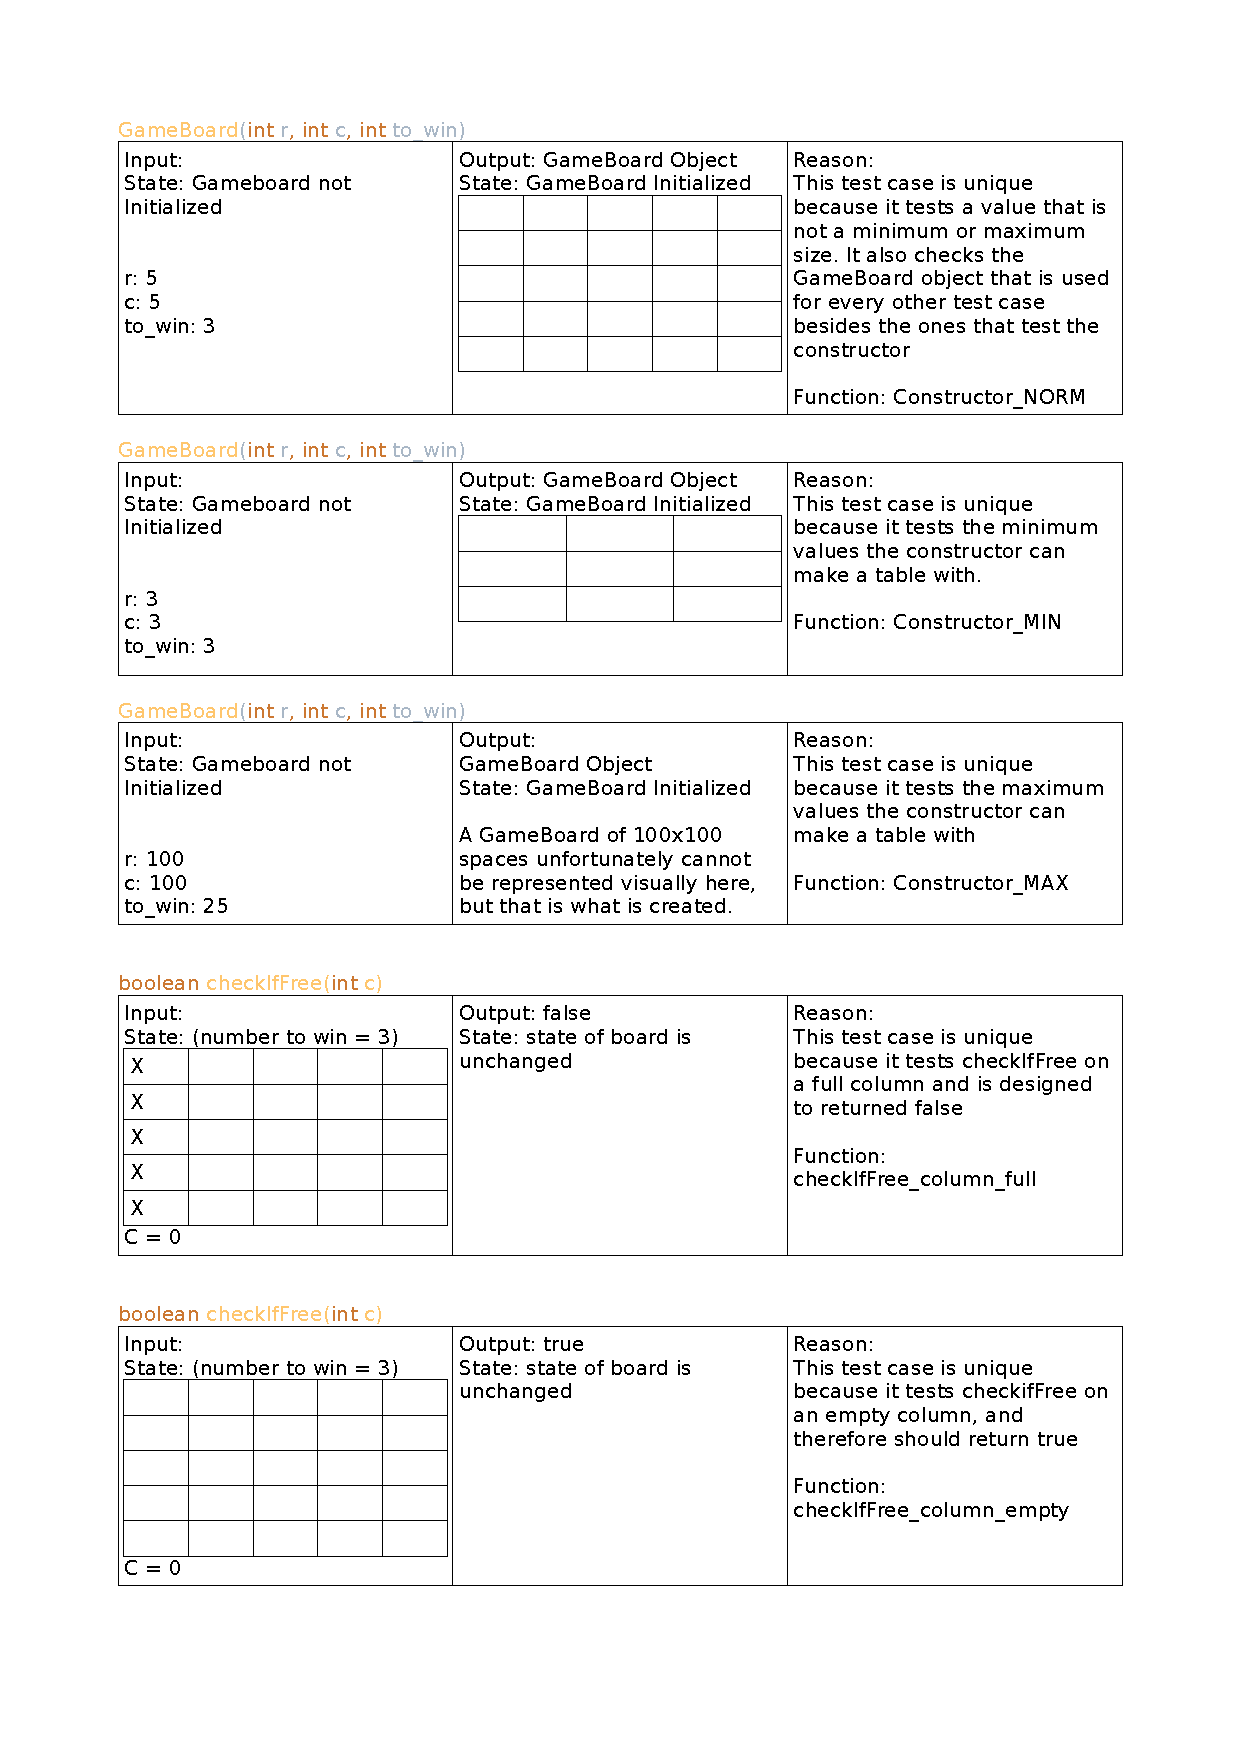
\includepdf[pages={1-10}]{test_cases}

\section{Deployment}
\paragraph{}
Untar the provided HW5.tar.gz

Run the ConnectXApp.java
\end{document}

